\documentclass[journal]{IEEEtran}
\usepackage[T1]{fontenc}
\usepackage{amsmath,amssymb,amsthm,mathtools}
\usepackage{booktabs}
\usepackage{graphicx}
\usepackage{xcolor}
\usepackage{algorithm}
\usepackage{algpseudocode}
\usepackage[numbers,sort&compress]{natbib}
\usepackage{microtype}
\usepackage{hyperref}
\hypersetup{colorlinks=true,linkcolor=blue!50!black,citecolor=blue!50!black,urlcolor=blue!50!black}

\newtheorem{theorem}{Theorem}
\newtheorem{proposition}{Proposition}
\newtheorem{lemma}{Lemma}
\newtheorem{corollary}{Corollary}
\theoremstyle{definition}
\newtheorem{definition}{Definition}
\newtheorem{assumption}{Assumption}

\newcommand{\R}{\mathbb{R}}
\newcommand{\E}{\mathbb{E}}
\newcommand{\cP}{\mathcal{P}}
\newcommand{\tr}{\operatorname{tr}}
\newcommand{\op}{\mathrm{op}}
\newcommand{\rhohat}{\hat\rho}
\DeclareMathOperator*{\argmax}{arg\,max}

\begin{document}
\title{DisCo-CFL: Calibrated, Fair and Explainable Clustered Federated Learning via Disattenuated Class-Conditional Gradient Signatures}
\author{Quang-Vinh~Dang%
\thanks{Q.-V. Dang is with British University Vietnam, Hung Yen, Vietnam (e-mail: vinh.dq4@buv.edu.vn; ORCID: 0000-0002-3877-8024).}}

\markboth{IEEE Transactions on Neural Networks and Learning Systems}{Dang: DisCo-CFL}
\maketitle

\begin{abstract}
Clustered federated learning (CFL) trains one model per group of clients that share a data distribution. Existing methods cluster high-dimensional, round-dependent updates or losses, tend to group clients by label distribution rather than by concept, fix the number of clusters by a hyperparameter without a stable meaning, degrade under quantity skew, and give no account of their grouping decisions. We propose DisCo-CFL. At a frozen reference model each client uploads, once, count-sketched mean gradients for every class it holds, computed on two random halves of that class. Spearman's correction for attenuation, estimated from the two halves, turns them into a \emph{calibrated} similarity. It is invariant to label and quantity skew by construction, consistent for the population cosine between class-conditional gradients even under differential-privacy noise, and equal to one for clients that share a concept. A class-wise bottleneck linkage with a single threshold then finds the number of clusters automatically. We prove safety (conflicting clients are never merged), maximality and exact recovery with a sample complexity that does not depend on cluster sizes, and a minimax lower bound that matches it up to a factor $1/\Delta$. We also prove differential privacy with an explicit cost, the fidelity of the class-level explanations the server produces, and the Bayes optimality of prior-corrected cluster models. The deterministic core of these proofs is machine-checked in Lean~4. DisCo-CFL also returns assignment certificates, an audit log and anomaly flags. On Fashion-MNIST, MNIST, SVHN and CIFAR-10 (618 runs, nine baselines), it recovers the groups without knowing $K$ (mean ARI $0.94$--$1.00$ in the rotation, label-swap, mixed and minority scenarios of Fashion-MNIST, MNIST and SVHN) and merges on average $0.1\%$ of the conflicting pairs there, against 8--84\% for baselines given $K$. It and is significantly better than every baseline on mean, concept and worst-group accuracy.
\end{abstract}

\begin{IEEEkeywords}
Federated learning, clustered federated learning, non-IID data, fairness, explainability, differential privacy, formal verification.
\end{IEEEkeywords}

\section{Introduction}
\IEEEPARstart{F}{ederated} learning (FL) trains models on data that never leave the clients~\cite{mcmahan2017fedavg,kairouz2021advances}. When client distributions differ, one global model can fit everyone poorly~\cite{zhao2018noniid}. Clustered FL (CFL) trains one model per group of clients with a common distribution~\cite{sattler2021cfl,ghosh2020ifca,briggs2020flhc}. A recent survey~\cite{benali2026survey} organises CFL into server-side, client-side and metadata-based methods, and it lists open problems that motivate this work:
\begin{itemize}
\item \emph{Clustering signal.} Server-side methods compare high-dimensional updates whose geometry changes from round to round, and CFL methods often group clients by \emph{label} similarity~\cite{guo2024fedrc}, which fragments data even when clients share a concept.
\item \emph{Number of clusters.} Every method depends on a hyperparameter that controls $K$ directly or indirectly; stable automatic determination remains open~\cite{benali2026survey}.
\item \emph{Quantity skew} is rarely evaluated, although existing CFL algorithms struggle with it~\cite{benali2025cornflqs}.
\item \emph{Privacy.} Metadata-based methods gain efficiency by sharing statistics with a moderate to high privacy risk, and formal privacy of the clustering signal is rare.
\item \emph{Evaluation beyond accuracy.} The quality of the grouping decision, its fairness towards small groups and its explainability to participants are hardly studied.
\end{itemize}

At a fixed reference model $w$, the expected gradient of the loss restricted to class $c$ depends on a client only through its class-conditional distribution $\cP_i(X\mid Y=c)$. It is therefore unaffected by label proportions and dataset size. Both kinds of concept shift change it: rotated inputs change $\cP(X\mid Y=c)$ for every class, and swapped labels change it for the swapped classes. Estimated class-conditional gradients are noisy, however, and noise \emph{attenuates} cosine similarities: two clients with the same concept but few samples look dissimilar. We correct this with Spearman's correction for attenuation~\cite{spearman1904,brown1910}. Each client splits each class into two halves; the agreement between the halves estimates the reliability of the signature, and dividing the cross-client cosine by the reliabilities yields the \emph{population} similarity. On this scale, $1$ means ``same concept'' for every client, whatever its data size or privacy noise.

Our contributions are as follows.
\begin{itemize}
\item \emph{Algorithm.} DisCo-CFL is a one-shot server-side CFL algorithm built on sketched class-conditional gradient signatures, split-half disattenuation, and threshold clustering with a class-wise bottleneck linkage and evidence-ordered merging. $K$ follows from one threshold on a calibrated scale (Section~\ref{sec:method}).
\item \emph{Theory.} We prove invariance, concentration, safety, maximality and exact recovery with a group-size-independent sample complexity, a minimax lower bound, differential privacy with an explicit cost, explanation fidelity, and Bayes optimality of prior-corrected cluster models. The deterministic core of every proof is machine-checked in Lean~4 (Section~\ref{sec:theory}).
\item \emph{Properties beyond accuracy.} The method provides minority protection, per-client assignment certificates, an audit log, anomaly flags, class-level explanations and an automatic heterogeneity diagnosis (Section~\ref{sec:fat}).
\item \emph{Evaluation.} We test on four datasets against nine baselines that cover all CFL families, with clustering, fairness, explanation and certificate metrics, robustness sweeps and significance tests (Section~\ref{sec:exp}).
\end{itemize}
Code, raw results and the Lean project are available at \url{https://github.com/vinhqdang/cluster_federated_learning}. Full statements, proofs, the Lean summary and additional results are in the supplementary material (Sections~S1--S4).

\section{Related Work and Positioning}\label{sec:related}
We follow the taxonomy of~\cite{benali2026survey}, which separates \emph{core} CFL (several models for statistical heterogeneity) from operational uses of clustering.

\emph{Server-side CFL} clusters updates or weights: trimmed $k$-means~\cite{ghosh2019robust}, recursive cosine bipartitioning (CFL/MTCFL)~\cite{sattler2021cfl}, one-shot hierarchical clustering (FL+HC)~\cite{briggs2020flhc}, SVD-reduced similarities~\cite{duan2021flexcfl,yan2023icfl}, EM in parameter space (FeSEM)~\cite{long2023fesem} and frozen-model gradients (StoCFL)~\cite{zeng2025stocfl}. Their common signal is a whole-model update, whose geometry changes across rounds, mixes label proportions with concepts and depends on the client's sample size. \emph{Client-side CFL} lets clients choose among $K$ models by loss (IFCA)~\cite{ghosh2020ifca,mansour2020three} or learn soft memberships~\cite{li2021flsc,ruan2022fedsoft,marfoq2021fedem,guo2024fedrc,guo2025hcfl}. These methods need a fixed or initial $K$, download $K$ models per round and are sensitive to initialisation. Loss-based assignment also reacts to label proportions: a client with a concentrated label mix prefers the model trained on a similar mix. \emph{Metadata-based CFL} shares data statistics such as centroids~\cite{dennis2021kfed}, subspaces (PACFL)~\cite{vahidian2023pacfl} or noisy label distributions~\cite{luo2024ppcfl}; the survey rates most of these as a moderate to high privacy risk~\cite{benali2026survey}. Closest to our work, FedDAG~\cite{pramanik2026feddag} fuses gradient similarity with class-wise principal angles between \emph{data} subspaces and selects $K$ with a compactness criterion, FedCCFA~\cite{chen2024fedccfa} clusters class-specific classifier vectors under concept drift, and CORNFLQS~\cite{benali2025cornflqs} alternates weight- and loss-based clustering for quantity skew. DisCo-CFL shares the view that concepts are best compared class by class, but it compares expected class-conditional gradients at a frozen model, which are functionals of $\cP(X\mid Y)$ alone. It also removes the noise-induced attenuation of the similarity, so the population value for clients that share a concept is exactly one. Multi-task learning groups tasks by gradient affinity~\cite{fifty2021tag,yu2020pcgrad}, and Spearman's correction is standard in psychometrics~\cite{spearman1910,muchinsky1996attenuation}; neither has been used to calibrate client similarities in FL, to our knowledge. Personalised FL~\cite{tan2022pflsurvey,li2021ditto,collins2021fedrep,fallah2020perfedavg} adapts one model per client, logit calibration counters label skew in a single model~\cite{zhang2022fedlc,menon2021logit}, and fair FL equalises accuracy across clients~\cite{li2020qffl,mohri2019afl}. In CFL, unfairness appears earlier, in the grouping itself: small groups can be absorbed and small clients isolated. Explanations that let an affected party understand and contest an automated decision~\cite{wachter2018counterfactual,doshivelez2017interpretable} have not been provided for client grouping, to our knowledge. Table~\ref{tab:position} positions DisCo-CFL. To our knowledge it is the first CFL method whose similarity is calibrated across sample sizes and privacy noise and invariant to label and quantity skew by construction. It is also the first to come with size-independent recovery guarantees, a matching lower bound checked in Lean~4, and explanations and certificates of the grouping decision.

\begin{table}[t]
\centering
\caption{Positioning. Cat.: server-/client-side/metadata. LS: invariant to label skew by design. QS: treats quantity skew. Priv.: formal privacy of the clustering signal. Expl./Cert.: explanations/certificates of the grouping. ``--'': not claimed as far as we could verify.}\label{tab:position}
\scriptsize\setlength{\tabcolsep}{2pt}
\resizebox{\columnwidth}{!}{%
\begin{tabular}{llllcccc}
\toprule
Method & Cat. & Clusters on & $K$ & LS & QS & Priv. & Expl./Cert. \\
\midrule
CFL~\cite{sattler2021cfl} & S & updates & threshold & -- & -- & -- & -- \\
FL+HC~\cite{briggs2020flhc} & S & updates & threshold & -- & -- & -- & -- \\
FeSEM~\cite{long2023fesem} & S & weights & fixed & -- & -- & -- & -- \\
IFCA~\cite{ghosh2020ifca} & C & local losses & fixed & -- & -- & -- & -- \\
FedRC~\cite{guo2024fedrc} & C & local losses & fixed & -- & -- & -- & -- \\
PACFL~\cite{vahidian2023pacfl} & M & data subspaces & threshold & -- & -- & -- & -- \\
pp-CFL~\cite{luo2024ppcfl} & M & noisy label dist. & COPRA & -- & -- & DP & -- \\
CORNFLQS~\cite{benali2025cornflqs} & S+C & weights, losses & iterative & -- & \checkmark & -- & -- \\
FedCCFA~\cite{chen2024fedccfa} & S & class classifiers & DBSCAN & partial & -- & -- & -- \\
FedDAG~\cite{pramanik2026feddag} & S+M & grads, subspaces & selected & partial & weights & -- & -- \\
\midrule
\textbf{DisCo-CFL} & S & class-cond.\ grads & calibrated & \checkmark & \checkmark & DP & \checkmark/\checkmark \\
\bottomrule
\end{tabular}}
\end{table}

\section{Problem Setting}\label{sec:setting}
Client $i\in[N]$ holds $n_i$ samples from $\cP_i(X,Y)=\cP_i(Y)\,\cP_i(X\mid Y)$ with labels in $[C]$; $S_i$ is the set of classes it holds with at least $m$ samples.
\begin{definition}[Conflicts]\label{def:concept}
Clients $i,j$ \emph{conflict on} $c\in S_i\cap S_j$ if $\cP_i(X\mid Y=c)\neq\cP_j(X\mid Y=c)$, and are \emph{compatible} otherwise. Clients belong to latent concept groups $G_1,\dots,G_K$ with shared class-conditionals.
\end{definition}
If $\cP_i(X\mid Y)=\cP_j(X\mid Y)$, the Bayes classifiers of $i$ and $j$ differ only through their label priors, which a shared model absorbs by prior correction~\cite{lipton2018labelshift,menon2021logit}. Label skew and quantity skew should therefore not create clusters, while concept shift on features or targets should.

\section{DisCo-CFL}\label{sec:method}
\emph{Signatures (client side).} After $T_0$ FedAvg warm-up rounds, the server broadcasts the reference model $w$ and the seed of a count-sketch $\Phi:\R^d\to\R^p$~\cite{charikar2002countsketch} ($p=1024$). With $g(x,c)=\operatorname{clip}_{C_{\rm clip}}(\Phi\nabla_w\ell(w;x,c))$, client $i$ splits the samples of each class $c\in S_i$ into halves $A_i^c,B_i^c$ of size $h_i^c$ and uploads, once,
\begin{equation*}
a_i^c=\tfrac1{h_i^c}\textstyle\sum_{s\in A_i^c}g(x_s,c),\qquad b_i^c=\tfrac1{h_i^c}\textstyle\sum_{s\in B_i^c}g(x_s,c).
\end{equation*}
Clipping ($C_{\rm clip}=0.5$) bounds heavy-tailed per-sample gradients and preserves invariance. For differential privacy, Gaussian noise is added to each half-mean.

\emph{Disattenuated similarity (server side).} With $m_i^c=(a_i^c+b_i^c)/2$, the split-half reliability and its Spearman--Brown extension are $r_i^c=\cos(a_i^c,b_i^c)$ and $R_i^c=2r_i^c/(1+r_i^c)$ ($R_i^c=0$ if $r_i^c\le0$). The calibrated similarity and its evidence weight are
\begin{equation}\label{eq:disatt}
\rhohat_{ij}^c=\operatorname{clip}_{[-1,1]}\!\Big(\frac{\cos(m_i^c,m_j^c)}{\sqrt{R_i^cR_j^c}}\Big),\qquad W_{ij}^c=R_i^cR_j^c .
\end{equation}

\emph{Clustering.} For client sets $A,B$ let $\mathrm{num}^c_{AB}=\sum_{i\in A,j\in B}W^c_{ij}\rhohat^c_{ij}$ and $\mathrm{den}^c_{AB}=\sum W^c_{ij}$. The bottleneck linkage is
\begin{equation}\label{eq:link}
L(A,B)=\min_c\frac{\mathrm{num}^c_{AB}+\lambda}{\mathrm{den}^c_{AB}+\lambda}\quad\text{if }\textstyle\sum_c\mathrm{den}^c_{AB}\ge e_{\min}.
\end{equation}
The minimum over classes encodes concept equivalence: two groups share a concept only if every class-conditional gradient agrees, so a label swap on 2 of 10 classes is not averaged away. The shrinkage $\lambda$ pulls classes with little evidence towards $1$ (no evidence of a difference). Starting from singletons, the server repeatedly merges, among the pairs with $L\ge\tau$, the pair with the \emph{largest shared evidence}, and stops when none is left. Evidence ordering lets well-supported groups form first, so that ambiguous clients (with little data on the discriminative classes) join them instead of bridging different groups. Because the scale is calibrated, $\tau$ has a fixed meaning; we use $\tau=0.8$, $\lambda=0.5$ everywhere. Clients with little evidence and singletons that are not significantly separated are attached to their closest cluster; significant singletons are kept and flagged as anomalous. Each cluster then runs FedAvg from $w$ (Algorithm~\ref{alg:disco}).

\emph{Inference.} Members of a cluster share class-conditionals but may have very different label proportions. Client $i$ therefore predicts with the prior-corrected cluster model
\begin{equation}\label{eq:pc}
\hat y(x)=\argmax_y\big[f_k(x)_y+\log\hat p_i(y)-\log\hat p_k(y)\big],
\end{equation}
where $f_k$ are the cluster model's logits, $\hat p_i$ is the client's label distribution and $\hat p_k$ the cluster's, a sum of counts that secure aggregation~\cite{bonawitz2017secagg} can provide. Label skew is thus handled by the prior rather than by more clusters. In the experiments the same correction is applied to every method.

\emph{Accountability and transparency outputs.} For every pair of clusters the server reports the \emph{divergent classes} $\hat D_{AB}=\{c:\rho^c_{AB}<\tau\}$. From them it diagnoses a global shift (all shared classes differ), a class-specific shift, or label and quantity skew only ($\hat K=1$). Each client receives an \emph{assignment certificate}: its bottleneck similarity to its own and to the closest other cluster, with standard errors and a verdict (confident, uncertain or low-evidence). Every merge and attachment decision is logged. Newcomers are assigned with the frozen $w$ or reported as a novel concept.

\begin{algorithm}[t]
\caption{DisCo-CFL}\label{alg:disco}
\small
\begin{algorithmic}[1]
\State $T_0$ rounds of FedAvg $\to$ reference $w$; broadcast $w$ and sketch seed
\State Each client uploads $(a_i^c,b_i^c)$ for $c\in S_i$ (clipped; noised if DP)
\State Server: $R_i^c$, $\rhohat^c_{ij}$, $W^c_{ij}$ by~\eqref{eq:disatt}; clusters $\gets$ singletons
\While{$\exists A,B$ with $L(A,B)\ge\tau$} merge the eligible pair of largest evidence; log \EndWhile
\State Attach low-evidence clients and non-significant singletons; flag anomalies
\State Output clusters, certificates, explanations, log; FedAvg per cluster from $w$
\end{algorithmic}
\end{algorithm}

\section{Theory}\label{sec:theory}
Let $\mu_i^c=\E_{x\sim\cP_i(X\mid Y=c)}[g(x,c)]$, $\rho_{ij}^c=\cos(\mu_i^c,\mu_j^c)$ and $a_i^c=\|\mu_i^c\|^2$. Proofs are in the supplementary material (Section~S2). The deterministic parts of all results below (25 theorems) are machine-checked in Lean~4 with Mathlib~\cite{moura2021lean4,mathlib2020}, without \texttt{sorry} and with only Lean's standard axioms (Section~S3). The probabilistic tools (Hanson--Wright, Bretagnolle--Huber, the analytic Gaussian mechanism) enter as cited hypotheses.

\begin{proposition}[Invariance]\label{prop:inv}
$\mu_i^c$ depends on client $i$ only through $\cP_i(X\mid Y=c)$. Compatible clients have $\rho^c_{ij}=1$ on every shared class, whatever their label proportions and sample sizes.
\end{proposition}
\begin{assumption}\label{ass:noise}
Per-sample signatures are $g=\mu_i^c+\Sigma^{1/2}z$ with independent $K_0$-sub-Gaussian coordinates of $z$; $\sigma^2=\tr\Sigma$, $r_s=\tr\Sigma/\|\Sigma\|_\op$, $r_e=(\tr\Sigma)^2/\|\Sigma\|_F^2$.
\end{assumption}
\begin{assumption}\label{ass:sep}
If $i,j$ conflict on $c$, then $\rho^c_{ij}\le1-\Delta$ for some $\Delta\in(0,1]$.
\end{assumption}
For a pair and class, let $h=\min(h_i^c,h_j^c)$, $a=\min(a_i^c,a_j^c)$ and $\kappa=\sigma^2/(ah)$.
\begin{theorem}[Calibration and concentration]\label{thm:conc}
In expectation, \eqref{eq:disatt} equals $\rho_{ij}^c$ exactly, for any noise levels. Under Assumption~\ref{ass:noise} with $\kappa\le1$, if $\eta:=(\sqrt{\kappa/r_s}+\kappa/\sqrt{r_e})\sqrt{\log(12/\delta)}\le c_0$, then $|\rhohat^c_{ij}-\rho^c_{ij}|\le C_1\eta$ with probability $1-\delta$. The raw cosine instead tends to $\rho^c_{ij}\sqrt{R_iR_j}$, which is biased towards $0$.
\end{theorem}
\begin{theorem}[Safety, maximality, recovery]\label{thm:rec}
Let $\gamma=\min(1-\tau,\tau-1+\Delta)>0$. If all estimates are within $\gamma/2$ of their targets and conflicting pairs have evidence $W^c_{ij}>2\lambda(1-\tau)/\gamma$, then for \emph{any} merge order: (a) no cluster contains conflicting clients; (b) any two output clusters sharing evidence $\ge e_{\min}$ contain a conflicting pair; (c) if every client holds all discriminative classes, the output equals $\{G_1,\dots,G_K\}$ and $\hat K=K$.
\end{theorem}
\begin{corollary}[Sample complexity, minority fairness]\label{cor:sc}
With $\mathsf L=\log(12N^2C/\delta)$, $\gamma\le1/3$ and $\lambda<\gamma/(8(1-\tau))$, Theorem~\ref{thm:rec} holds with probability $1-\delta$ if every half size satisfies
\begin{equation*}
h\ge h^\star=C_2\frac{\sigma^2}{a}\max\Big\{\frac{\mathsf L}{r_s\gamma^2},\frac{\sqrt{\mathsf L}}{\sqrt{r_e}\,\gamma},1\Big\}.
\end{equation*}
$h^\star$ does not depend on the group sizes: a single-client concept is recovered under the same condition as a large group.
\end{corollary}
\begin{theorem}[Minimax lower bound]\label{thm:lb}
With Gaussian noise, any test deciding $\rho_{ij}=1$ versus $\rho_{ij}=1-\Delta$ from $n$ samples has error at least $\frac14\exp(-na\Delta r_s/\sigma^2)$, so error $\delta$ requires $n\ge\frac{\sigma^2}{ar_s\Delta}\log\frac1{4\delta}$.
\end{theorem}
With $\gamma=\Delta/2$ the upper bound is $O(\sigma^2\mathsf L/(ar_s\Delta^2))$. The two bounds agree in $\sigma^2$, $a$ and $r_s$, and differ by a factor $1/\Delta$ and a $\log N$ term.
\begin{proposition}[Privacy]\label{prop:dp}
With per-sample clipping and Gaussian noise of multiplier $\sigma_{\rm dp}$, each half-mean has replace-one sensitivity $2C_{\rm clip}/h$. The signature is therefore $(\varepsilon,\delta)$-DP given the labels (analytic Gaussian mechanism~\cite{balle2018analytic}, parallel composition). Theorem~\ref{thm:conc} still holds, with an additional requirement $h\gtrsim\sigma_{\rm dp}C_{\rm clip}\sqrt{\mathsf L}/(\sqrt a\gamma)$ that is linear in $1/\varepsilon$. The raw cosine collapses unless $h\gg\sqrt p\,\sigma_{\rm dp}C_{\rm clip}/\sqrt a$.
\end{proposition}
\begin{proposition}[Explanations and prior correction]\label{prop:expl}
Under the conditions of Theorem~\ref{thm:rec}, $c\in\hat D_{AB}$ if and only if the concepts of $A$ and $B$ differ on $c$. For concept-equivalent clients, $\cP_i(y\mid x)\propto q_k(y\mid x)\cP_i(y)/\cP_k(y)$, so the prior-corrected cluster model is Bayes-optimal for every member, and no finer clustering reduces its Bayes risk.
\end{proposition}

\emph{Proof sketches.} For Theorem~\ref{thm:conc}, the expectations of the split-half inner product and norms are $a_i$ and $a_i+t_i$, where $t_i$ is the half-mean noise trace. Hence $R_i^\star=a_i/(a_i+t_i/2)$, $\E\|m_i\|^2=a_i/R_i^\star$, and the attenuation factor cancels exactly. Concentration follows from sub-Gaussian bounds for the linear noise terms and Hanson--Wright~\cite{rudelson2013hansonwright} for the quadratic ones, combined with the smoothness of the estimator. For Theorem~\ref{thm:rec}, if two conflict-free clusters contain a conflicting pair on class $c$, then \emph{all} their cross pairs that hold $c$ conflict. The pooled class term is then at most $(\mathrm{den}(1-\Delta+\gamma/2)+\lambda)/(\mathrm{den}+\lambda)<\tau$ once the evidence exceeds $w_0$, so conflicting clusters are never linked, whatever the merge order. Conversely, compatible clusters have every class term at least $(1+\tau)/2>\tau$, which gives maximality. Under full support, conflict-freeness forces purity, and maximality forces one cluster per group. Theorem~\ref{thm:lb} is a two-point Le Cam argument: the two hypotheses differ along the top eigenvector of $\Sigma$, and their KL divergence is $na\Delta r_s/\sigma^2$.

\emph{Scope.} Theorem~\ref{thm:rec} covers the merging phase and any merge order. The attachment of low-evidence clients and non-significant singletons is a fairness heuristic that avoids training a client alone because of noise; it is logged in the audit trail. Clients that hold none of the discriminative classes are compatible with several groups and may join any of them, which is harmless for training but lowers ARI.

\section{Fairness, Accountability, Transparency and Privacy}\label{sec:fat}
\emph{Fairness.} By Corollary~\ref{cor:sc}, recovery does not depend on group size. By contrast, $k$-means-type objectives favour large clusters, and IFCA's analysis depends on the smallest cluster fraction~\cite{ghosh2020ifca}. Small clients are not pushed away by attenuation (Theorem~\ref{thm:conc}), and merely noisy clients are attached rather than isolated. \emph{Accountability.} Certificates, the audit log and anomaly flags make each grouping decision traceable and contestable; newcomers are handled with the same frozen model. \emph{Transparency.} Participants learn \emph{why} they were separated (``you differ from cluster 2 on classes 3 and 5''), with a fidelity guarantee (Proposition~\ref{prop:expl}). \emph{Privacy.} Proposition~\ref{prop:dp} gives record-level DP for the only extra information released: a low-dimensional sketch, uploaded once.

\section{Experiments}\label{sec:exp}
\begin{table}[t]
\centering
\caption{Scenarios (3 seeds each). QS: quantity skew; part.: fraction of clients per round.}\label{tab:scen}
\scriptsize\setlength{\tabcolsep}{2.5pt}
\begin{tabular}{llll}
\toprule
Scenario & Datasets & Concept groups & Notes \\
\midrule
Rotation & all four & 4 rotations ($90^\circ$ steps) & 40 clients \\
Label swap & all four & 4 labelings (2 swapped pairs) & 40 clients \\
Rot.+QS, Mixed+QS & FMNIST & rotations / 2 rot.\ $\times$ 2 lab. & log-normal sizes \\
Label only & FMNIST & 1 (true $K=1$) & $\alpha=0.1$, QS \\
Minority & FMNIST & 4 rotations, 25/9/4/2 clients & \\
Strength & FMNIST & rotations by $0,\theta,2\theta,3\theta$ & $\theta\in\{15,30,45\}^\circ$ \\
Groups & FMNIST & $K\in\{2,4,8\}$ labelings & \\
Participation & FMNIST & rotation / label swap & part.\ $=0.3$ \\
Scale & FMNIST & 4 rotations & 200 clients \\
\bottomrule
\end{tabular}
\end{table}

\emph{Setup.} We use Fashion-MNIST~\cite{xiao2017fmnist}, MNIST~\cite{lecun1998mnist}, SVHN~\cite{netzer2011svhn} and CIFAR-10~\cite{krizhevsky2009cifar}, with 40 clients in four concept groups unless stated. \emph{Rotation} applies a concept shift on features ($0^\circ$--$270^\circ$); \emph{label swap} applies a concept shift on targets (two swapped class pairs per group). All clients have Dirichlet label skew ($\alpha=0.3$), and some scenarios add quantity skew (QS, log-normal sizes). \emph{Mixed + QS} combines two rotations with two labelings; \emph{Label only} has a single concept ($K=1$, $\alpha=0.1$); \emph{Minority} has groups of 25/9/4/2 clients. All methods use the same CNN (47k parameters; 66k for colour images), SGD with learning rate 0.05, one local epoch and 50 rounds; methods with a warm-up use 10 of them. Baselines: FedAvg~\cite{mcmahan2017fedavg}, Local, FedAvg with fine-tuning (FT), IFCA~\cite{ghosh2020ifca}, FeSEM~\cite{long2023fesem}, CFL~\cite{sattler2021cfl}, FL+HC~\cite{briggs2020flhc}, PACFL~\cite{vahidian2023pacfl} and an Oracle trained on the true groups. IFCA, FeSEM, FL+HC and PACFL are given the true $K$. Accuracy (Acc) is the mean local test accuracy with the same prior correction for every method. \emph{Concept accuracy} (Con.) is measured on a class-balanced test set of the client's concept. The \emph{conflict-merge rate} is the fraction of conflicting pairs placed in one cluster. DisCo-CFL uses $p=1024$, $\tau=0.8$, $\lambda=0.5$, $e_{\min}=0.05$, $C_{\rm clip}=0.5$ and $z=2$ everywhere. These values were fixed on seed 0 of four pilot scenarios using clustering quality only; all other seeds, the sweeps and the MNIST, SVHN and CIFAR-10 results were unseen during design. The CFL thresholds and the FeSEM initialisation (warm-up and $k$-means++ seeding) were selected on the same pilot run. Without them, CFL never splits and FeSEM collapses to one cluster. We report 3 seeds per configuration, 618 runs in total. Full tables with standard deviations and fairness metrics are in Section~S4.

\begin{table*}[t]
\centering
\caption{Fashion-MNIST: mean local accuracy (Acc) and concept accuracy (Con.) in \%, 3 seeds, with prior correction for all methods. Best non-oracle value in bold.}\label{tab:fmnist}
\footnotesize
\begin{tabular}{lcccccccccccc}
\toprule
 & \multicolumn{2}{c}{Rotation} & \multicolumn{2}{c}{Label swap} & \multicolumn{2}{c}{Rot.+QS} & \multicolumn{2}{c}{Mixed+QS} & \multicolumn{2}{c}{Label only} & \multicolumn{2}{c}{Minority} \\
\cmidrule(lr){2-3}\cmidrule(lr){4-5}\cmidrule(lr){6-7}\cmidrule(lr){8-9}\cmidrule(lr){10-11}\cmidrule(lr){12-13}
Method & Acc & Con. & Acc & Con. & Acc & Con. & Acc & Con. & Acc & Con. & Acc & Con. \\
\midrule
FedAvg & 86.0 & 75.7 & 70.1 & 55.7 & 85.8 & 74.7 & 80.8 & 66.6 & 95.5 & 85.8 & 85.5 & 76.7 \\
Local & 87.8 & 60.7 & 88.7 & 64.0 & 87.9 & 61.9 & 88.9 & 64.1 & 94.6 & 51.0 & 88.5 & 62.7 \\
FedAvg-FT & 88.8 & 77.9 & 90.6 & 80.9 & 87.6 & 75.4 & 88.6 & 76.5 & 94.2 & 80.7 & 89.4 & 78.5 \\
IFCA & 89.2 & 77.0 & 85.6 & 71.1 & 88.5 & 77.0 & 89.0 & 75.4 & 95.4 & 85.7 & 89.4 & 78.1 \\
FeSEM & 89.1 & 80.6 & 87.5 & 79.8 & 88.3 & 78.4 & 88.1 & 77.9 & 95.5 & 85.7 & 89.8 & 81.8 \\
CFL & 90.2 & 73.9 & 90.4 & 76.1 & 88.8 & 73.5 & 84.8 & 70.2 & 95.3 & 77.1 & 87.3 & 76.7 \\
FL+HC & 86.4 & 74.9 & 71.5 & 59.1 & 85.3 & 73.5 & 81.8 & 67.1 & 95.5 & \textbf{85.9} & 87.7 & 78.0 \\
PACFL & 89.5 & 79.4 & 74.8 & 53.6 & 88.0 & 76.5 & 83.3 & 66.4 & 95.5 & 85.8 & 89.8 & 78.8 \\
\textbf{DisCo-CFL} & \textbf{90.5} & \textbf{83.9} & \textbf{90.8} & \textbf{84.9} & \textbf{90.1} & \textbf{82.1} & \textbf{90.6} & \textbf{82.5} & \textbf{95.6} & 85.6 & \textbf{90.8} & \textbf{84.1} \\
\midrule
Oracle & 90.5 & 83.9 & 90.8 & 84.9 & 90.1 & 82.1 & 90.6 & 83.4 & 95.5 & 85.8 & 90.9 & 84.2 \\
\bottomrule
\end{tabular}
\end{table*}

\begin{table*}[t]
\centering
\caption{MNIST, SVHN and CIFAR-10 (same metrics). DisCo-T30: DisCo-CFL with 30 warm-up rounds.}\label{tab:other}
\footnotesize
\begin{tabular}{lcccccccccccc}
\toprule
 & \multicolumn{2}{c}{MNIST rot.} & \multicolumn{2}{c}{MNIST swap} & \multicolumn{2}{c}{SVHN rot.} & \multicolumn{2}{c}{SVHN swap} & \multicolumn{2}{c}{CIFAR rot.} & \multicolumn{2}{c}{CIFAR swap} \\
\cmidrule(lr){2-3}\cmidrule(lr){4-5}\cmidrule(lr){6-7}\cmidrule(lr){8-9}\cmidrule(lr){10-11}\cmidrule(lr){12-13}
Method & Acc & Con. & Acc & Con. & Acc & Con. & Acc & Con. & Acc & Con. & Acc & Con. \\
\midrule
FedAvg & 94.7 & 90.6 & 78.5 & 60.9 & 72.4 & 63.4 & 64.5 & 50.9 & 55.1 & 36.8 & 51.0 & 33.5 \\
Local & 96.5 & 82.0 & 97.1 & 86.0 & 77.5 & 43.9 & 81.0 & 50.4 & 56.2 & 21.0 & 56.4 & 21.8 \\
FedAvg-FT & 97.2 & 94.6 & 98.1 & 92.0 & 81.9 & 69.5 & 84.9 & 72.7 & 61.8 & 36.8 & 64.5 & 40.8 \\
IFCA & 96.9 & 91.2 & 95.8 & 87.9 & 80.2 & 65.9 & 79.0 & 64.1 & 56.5 & 32.0 & 55.0 & 30.7 \\
FeSEM & 98.2 & 95.9 & 98.4 & 97.1 & 84.1 & 75.6 & 80.5 & 70.9 & 61.9 & \textbf{44.8} & 59.8 & 43.7 \\
CFL & 95.7 & 90.8 & 91.7 & 78.7 & 84.0 & 66.9 & 83.1 & 66.5 & \textbf{67.0} & 38.2 & \textbf{68.8} & 41.4 \\
FL+HC & 94.3 & 89.9 & 80.8 & 65.9 & 72.9 & 64.4 & 66.6 & 53.4 & 55.6 & 36.9 & 53.1 & 34.5 \\
PACFL & 96.8 & 91.6 & 83.3 & 63.4 & 78.1 & 67.5 & 69.1 & 48.2 & 58.6 & 37.3 & 52.0 & 29.9 \\
\textbf{DisCo-CFL} & \textbf{98.5} & \textbf{97.1} & \textbf{98.7} & \textbf{97.8} & \textbf{85.4} & \textbf{79.7} & \textbf{87.2} & \textbf{82.5} & 60.5 & 41.0 & 64.1 & 48.6 \\
DisCo-T30 & -- & -- & -- & -- & 84.6 & 78.6 & 87.1 & 82.1 & 62.0 & \textbf{44.8} & 64.6 & \textbf{49.8} \\
\midrule
Oracle & 98.5 & 97.2 & 98.7 & 97.8 & 85.5 & 80.0 & 87.1 & 82.6 & 64.2 & 47.4 & 64.7 & 49.6 \\
\bottomrule
\end{tabular}
\end{table*}

\emph{Clustering quality.} Table~\ref{tab:cluster} averages the clustering metrics over the concept-shift scenarios of each dataset. Without knowing $K$, DisCo-CFL recovers the groups on Fashion-MNIST, MNIST and SVHN (ARI $0.98$) and merges at most $0.1\%$ of conflicting pairs. The baselines given $K$ merge $3$--$85\%$. FeSEM is the strongest of them, and FL+HC groups clients by label mix. CFL reaches few conflicts only when it fragments the federation into up to 35 clusters.

\begin{table}[t]
\centering
\caption{Clustering: mean ARI and conflict-merge rate (Conf., \%) over the concept-shift scenarios of each dataset.}\label{tab:cluster}
\scriptsize\setlength{\tabcolsep}{2.5pt}
\begin{tabular}{lcccccccc}
\toprule
 & \multicolumn{2}{c}{FMNIST} & \multicolumn{2}{c}{MNIST} & \multicolumn{2}{c}{SVHN} & \multicolumn{2}{c}{CIFAR-10} \\
\cmidrule(lr){2-3}\cmidrule(lr){4-5}\cmidrule(lr){6-7}\cmidrule(lr){8-9}
Method & ARI & Conf. & ARI & Conf. & ARI & Conf. & ARI & Conf. \\
\midrule
IFCA & 0.44 & 22.3 & 0.51 & 17.5 & 0.32 & 23.5 & 0.03 & 29.6 \\
FeSEM & 0.70 & 8.3 & 0.88 & 3.0 & 0.67 & 11.1 & 0.67 & 11.7 \\
CFL & 0.21 & 22.9 & 0.17 & 41.5 & 0.27 & 10.6 & 0.16 & 0.3 \\
FL+HC & 0.05 & 83.2 & 0.01 & 85.3 & 0.01 & 84.9 & 0.01 & 85.0 \\
PACFL & 0.31 & 23.3 & 0.22 & 23.0 & 0.19 & 22.9 & 0.19 & 33.3 \\
\textbf{DisCo-CFL} & 0.98 & 0.1 & 0.98 & 0.0 & 0.98 & 0.0 & 0.63 & 13.8 \\
DisCo-CFL (30 warm-up) & -- & -- & -- & -- & -- & -- & 0.83 & 2.2 \\
\bottomrule
\end{tabular}
\end{table}

\emph{Performance and fairness.} On Fashion-MNIST, MNIST and SVHN, DisCo-CFL has the best accuracy in every scenario and the best concept accuracy in every concept-shift scenario, within $0.1$ points of the Oracle (Tables~\ref{tab:fmnist}--\ref{tab:other}). Local training, FT and CFL obtain competitive local accuracy by personalising to the label mix, but their concept accuracy is 4--23 points lower on Fashion-MNIST. With a single concept (\emph{Label only}) DisCo-CFL returns $K=1$ in two seeds; in the third it flags one anomalous client. For minority concepts, its worst-group accuracy is 86.5\%, against 35.7\% (FedAvg), 51.9\% (CFL), 67.3\% (IFCA) and 79.4\% (FeSEM). In the clustering step alone, minority groups of 1--5 clients are recovered with recall $1.00$ (Section~S4).

\emph{CIFAR-10.} With 10 warm-up rounds the reference model is weak (about 40\% accurate) and rotations are hard to separate (ARI $0.38$): the separation $\Delta$ is small, as the theory warns. With 30 warm-up rounds, ARI reaches $0.74$ and $0.92$ and concept accuracy is the best of all non-oracle methods (44.8\% and 49.8\%, tied with FeSEM on rotation). CFL keeps the best local accuracy on CIFAR-10 by fragmenting into 33--35 clusters, at 7--8 points lower concept accuracy.

\emph{Robustness sweeps} (Table~\ref{tab:sweep}). Varying the rotation step $\theta$, DisCo-CFL separates the groups from $30^\circ$ on. At $15^\circ$ it merges neighbouring concepts that it cannot tell apart (ARI $0.42$) and loses only $0.5$ points to the Oracle. With 2 or 8 groups, 30\% participation or 200 clients, it stays within $0.1$ points of the Oracle and 1.3--2.9 points above the best baseline.

\begin{table}[t]
\centering
\caption{Robustness sweeps (Fashion-MNIST): DisCo-CFL vs.\ best baseline and Oracle accuracy.}\label{tab:sweep}
\scriptsize\setlength{\tabcolsep}{2.5pt}
\begin{tabular}{lcccccc}
\toprule
Setting & ARI & $\hat K$ & Acc & Con. & Best base.\ Acc / Con. & Oracle \\
\midrule
$\theta{=}15^\circ$ & 0.42 & 3.0 & 90.0 & 82.8 & 90.2 / 83.0 & 90.5 \\
$\theta{=}30^\circ$ & 0.93 & 4.3 & 90.3 & 83.1 & 90.0 / 81.2 & 90.4 \\
$\theta{=}45^\circ$ & 1.00 & 4.0 & 90.4 & 83.8 & 89.9 / 81.8 & 90.4 \\
$K{=}2$ & 0.94 & 3.3 & 91.4 & 86.5 & 88.5 / 80.2 & 91.5 \\
$K{=}8$ & 0.92 & 8.0 & 90.4 & 81.7 & 88.0 / 75.4 & 90.5 \\
part.\ rot. & 1.00 & 4.0 & 89.1 & 78.4 & 87.5 / 75.1 & 89.1 \\
part.\ swap & 0.98 & 4.0 & 89.3 & 78.3 & 86.5 / 73.0 & 89.3 \\
$N{=}200$ & 0.98 & 6.3 & 91.1 & 86.6 & 89.8 / 83.9 & 91.1 \\
\bottomrule
\end{tabular}
\end{table}

\emph{Significance.} Table~\ref{tab:signif} compares DisCo-CFL with each baseline over all (scenario, seed) pairs with concept shift. One-sided Wilcoxon signed-rank tests find it better than every baseline on mean, concept and worst-group accuracy (all $p<0.01$). The closest competitors are FeSEM, CFL and FT, which win mainly on CIFAR-10 and at $\theta=15^\circ$.

\begin{table}[t]
\centering
\caption{Paired one-sided Wilcoxon signed-rank tests, DisCo-CFL vs.\ each baseline, over (scenario, seed) pairs with concept shift. W/T/L: wins/ties/losses of DisCo-CFL.}\label{tab:signif}
\scriptsize\setlength{\tabcolsep}{2.2pt}
\begin{tabular}{lrcccccc}
\toprule
& & \multicolumn{2}{c}{Acc} & \multicolumn{2}{c}{Con.} & \multicolumn{2}{c}{Worst-grp} \\
\cmidrule(lr){3-4}\cmidrule(lr){5-6}\cmidrule(lr){7-8}
Baseline & $n$ & W/T/L & $p$ & W/T/L & $p$ & W/T/L & $p$ \\
\midrule
FedAvg & 57 & 57/0/0 & 2.6e-11 & 57/0/0 & 2.6e-11 & 57/0/0 & 2.6e-11 \\
Local & 33 & 33/0/0 & 1.2e-10 & 33/0/0 & 1.2e-10 & 32/0/1 & 2.3e-10 \\
FedAvg-FT & 33 & 27/1/5 & 2.3e-5 & 33/0/0 & 1.2e-10 & 24/0/9 & 0.004 \\
IFCA & 54 & 54/0/0 & 8.1e-11 & 54/0/0 & 8.1e-11 & 54/0/0 & 8.1e-11 \\
FeSEM & 57 & 45/4/8 & 2.5e-8 & 48/2/7 & 1.4e-8 & 47/3/7 & 5.2e-8 \\
CFL & 39 & 30/2/7 & 0.002 & 39/0/0 & 1.8e-12 & 30/0/9 & 1.4e-4 \\
FL+HC & 57 & 57/0/0 & 2.6e-11 & 57/0/0 & 2.6e-11 & 57/0/0 & 2.6e-11 \\
PACFL & 57 & 54/0/3 & 7.0e-11 & 57/0/0 & 2.6e-11 & 53/1/3 & 5.1e-11 \\
\bottomrule
\end{tabular}
\end{table}

\emph{Transparency and accountability} (Table~\ref{tab:fat}). For label swaps, the divergent classes reported by the server are exactly the swapped classes in every cluster pair (precision and recall $1.00$). For rotations, precision is $1.00$ and recall $0.93$; every miss is a $0^\circ/180^\circ$ pair on items nearly invariant under that rotation. Confident certificates (93--97\% of clients) are conflict-free in 100\% of cases for rotation and swap and in 91.9\% for \emph{Mixed + QS}, against 77.8\% for uncertain ones. Newcomers are assigned correctly in 96--100\% of cases, and 100\% of novel-concept newcomers are flagged.

\begin{table}[t]
\centering
\caption{Transparency and accountability (Fashion-MNIST, 3 seeds).}\label{tab:fat}
\scriptsize\setlength{\tabcolsep}{3pt}
\begin{tabular}{lccc}
\toprule
& Rotation & Label swap & Mixed+QS \\
\midrule
Divergent classes: precision / recall & 1.00 / 0.93 & 1.00 / 1.00 & 1.00 / 0.92 \\
Confident certificates (share) & 0.95 & 0.97 & 0.93 \\
Conflict-free: confident / uncertain & 1.00 / 1.00 & 1.00 / 1.00 & 0.92 / 0.78 \\
Newcomers: known correct / novel flagged & 1.00 / 1.00 & 0.96 / 1.00 & -- \\
\bottomrule
\end{tabular}
\end{table}

\emph{Minority recovery.} In the clustering step alone (groups of 20/10/10/$m$ clients), DisCo-CFL recovers minority groups of $m=1,2,3,5$ clients with recall and purity $1.00$, ARI $0.98$--$1.00$ and no conflicting merge. FL+HC isolates the minority only by spending its fixed $K$ on it, while merging 81\% of the conflicting pairs among the majority groups. PACFL does not find the minority at all.

\emph{Privacy and calibration.} Under $(\varepsilon,10^{-5})$-DP signatures (Fig.~\ref{fig:dp}), the raw cosine collapses at every noise level, as Proposition~\ref{prop:dp} predicts. DisCo-CFL keeps ARI $0.92$ (rotation) and $0.77$ (swap) at $\varepsilon=4.4$ with 1,500 samples per client. The same-group similarity stays at $0.98$--$0.99$ for client sizes from 50 to 800 samples, $\tau\in[0.75,0.85]$ works in all concept-shift scenarios, and $\lambda$ has almost no effect between $0.02$ and $1$. The threshold study is shown in Fig.~\ref{fig:tau}. With the raw cosine, every $\tau$ above $0.7$ over-splits.

\begin{figure}[t]
\centering
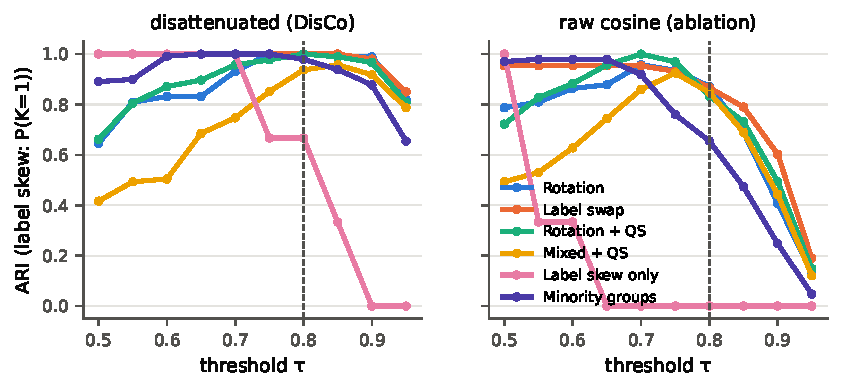
\includegraphics[width=\columnwidth]{tau_sensitivity.pdf}
\caption{ARI vs.\ threshold $\tau$ (label only: probability of $\hat K=1$). Left: DisCo-CFL; right: raw cosine. Dashed: default $\tau=0.8$, fixed before these runs.}\label{fig:tau}
\end{figure}

\emph{Ablation} (Table~\ref{tab:ablation}). Every component matters. Without class conditioning, clients cluster by label mix (13--23 clusters, the failure mode noted in~\cite{benali2026survey}). Without disattenuation, noise-attenuated similarities over-split the federation. The mean linkage averages class-specific shifts away and merges conflicting clients. Linkage-ordered merging creates bridges through ambiguous clients, and without clipping heavy-tailed gradients inflate $\hat K$.

\begin{table}[t]
\centering
\caption{Ablation (Fashion-MNIST, 3 seeds): ARI / number of clusters.}\label{tab:ablation}
\scriptsize\setlength{\tabcolsep}{2.5pt}
\begin{tabular}{lccccc}
\toprule
Variant & Rot. & Swap & Rot.+QS & Mixed+QS & Label only \\
\midrule
DisCo-CFL (full) & 1.00/4.0 & 1.00/4.0 & 1.00/4.0 & 0.94/4.0 & $\hat K$=1.3 \\
w/o disattenuation & 0.87/6.7 & 0.87/6.0 & 0.83/7.0 & 0.85/5.7 & $\hat K$=4.0 \\
w/o class conditioning & 0.15/23.3 & 0.15/17.7 & 0.16/22.3 & 0.09/22.3 & $\hat K$=13.0 \\
mean linkage & 1.00/4.0 & 0.80/4.0 & 0.92/4.0 & 0.69/4.0 & $\hat K$=1.0 \\
linkage-ordered merging & 0.95/5.0 & 0.86/5.7 & 1.00/4.0 & 0.81/5.7 & $\hat K$=1.7 \\
w/o clipping & 0.94/5.0 & 1.00/4.0 & 0.91/5.7 & 0.88/5.3 & $\hat K$=3.0 \\
\bottomrule
\end{tabular}
\end{table}

\emph{Theory in practice.} On synthetic signatures with known ground truth ($p=512$, noise of effective rank 16; Fig.~\ref{fig:theory}), safety and exact recovery are reached with probability one once $h\ge64$ for every $\Delta\in[0.2,0.7]$, independently of the minority size, as Corollary~\ref{cor:sc} states. The disattenuated similarity is nearly unbiased for every half size, whereas the raw cosine is biased by up to $-0.37$.

\begin{figure}[t]
\centering
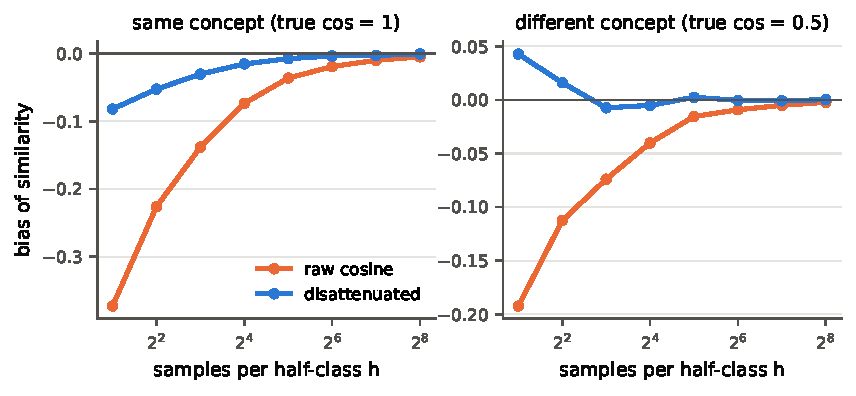
\includegraphics[width=\columnwidth]{theory_estimation.pdf}\\[2pt]
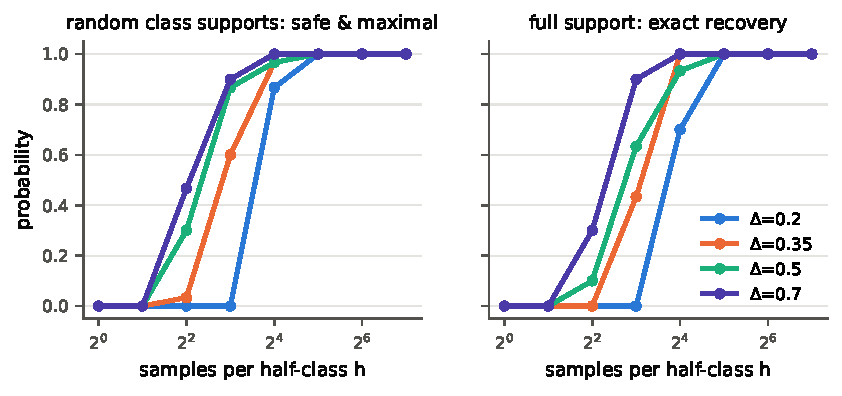
\includegraphics[width=\columnwidth]{theory_recovery.pdf}
\caption{Synthetic validation. Top: bias of the similarity (raw cosine vs.\ disattenuated) for same and different concepts. Bottom: probability of safety and maximality (left) and of exact recovery under full support (right) vs.\ half size $h$ (Theorem~\ref{thm:rec}).}\label{fig:theory}
\end{figure} Each client uploads about $1.2\times10^4$ floats once, and server clustering takes 2.3\,s for 320 clients.

\begin{figure}[t]
\centering
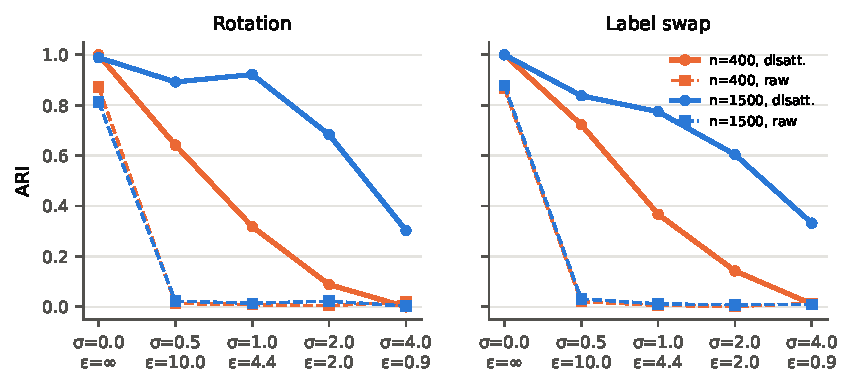
\includegraphics[width=\columnwidth]{dp.pdf}
\caption{Clustering ARI under $(\varepsilon,10^{-5})$-DP signatures. Solid: DisCo-CFL; dashed: raw cosine; 400 (orange) or 1,500 (blue) samples per client.}\label{fig:dp}
\end{figure}

\section{Discussion and Conclusion}
DisCo-CFL replaces heuristic client similarities with a statistic whose value for clients that share a concept is known in advance, namely one. Invariance to label and quantity skew, an automatic $K$, size-independent recovery, robustness to privacy noise and faithful explanations all follow from this calibration. Assignment certificates, the audit log and anomaly flags extend the evaluation of CFL from accuracy to fairness, accountability, transparency and privacy.

The method has limitations.
\begin{enumerate}
\item The class supports and half sizes are revealed to the server; the DP guarantee protects records given the labels.
\item The analysis assumes sub-Gaussian signatures and a fixed reference model, does not cover the attachment heuristics, and leaves a factor $1/\Delta$ between the upper and lower bounds.
\item Shifts that leave the reference-model gradient unchanged are invisible (e.g.\ $180^\circ$ rotations of symmetric items), and a weak reference model reduces separation, as on CIFAR-10 with a short warm-up.
\item Clustering is one-shot. Drift after clustering requires new signatures, although newcomers with unseen concepts are already detected.
\item The experiments use small CNNs and synthetic concept groups, as is standard in CFL~\cite{benali2026survey}.
\end{enumerate}
Adaptive warm-up, natural federated datasets and larger models are the next steps.

% Generated by IEEEtranN.bst, version: 1.14 (2015/08/26)
\begin{thebibliography}{51}
\providecommand{\natexlab}[1]{#1}
\providecommand{\url}[1]{#1}
\csname url@samestyle\endcsname
\providecommand{\newblock}{\relax}
\providecommand{\bibinfo}[2]{#2}
\providecommand{\BIBentrySTDinterwordspacing}{\spaceskip=0pt\relax}
\providecommand{\BIBentryALTinterwordstretchfactor}{4}
\providecommand{\BIBentryALTinterwordspacing}{\spaceskip=\fontdimen2\font plus
\BIBentryALTinterwordstretchfactor\fontdimen3\font minus
  \fontdimen4\font\relax}
\providecommand{\BIBforeignlanguage}[2]{{%
\expandafter\ifx\csname l@#1\endcsname\relax
\typeout{** WARNING: IEEEtranN.bst: No hyphenation pattern has been}%
\typeout{** loaded for the language `#1'. Using the pattern for}%
\typeout{** the default language instead.}%
\else
\language=\csname l@#1\endcsname
\fi
#2}}
\providecommand{\BIBdecl}{\relax}
\BIBdecl

\bibitem[McMahan et~al.(2017)McMahan, Moore, Ramage, Hampson, and Ag{\"u}era~y
  Arcas]{mcmahan2017fedavg}
B.~McMahan, E.~Moore, D.~Ramage, S.~Hampson, and B.~Ag{\"u}era~y Arcas,
  ``Communication-efficient learning of deep networks from decentralized
  data,'' in \emph{Proceedings of the 20th International Conference on
  Artificial Intelligence and Statistics (AISTATS)}, ser. PMLR, vol.~54, 2017,
  pp. 1273--1282.

\bibitem[Kairouz et~al.(2021)Kairouz, McMahan, et~al.]{kairouz2021advances}
P.~Kairouz, H.~B. McMahan \emph{et~al.}, ``Advances and open problems in
  federated learning,'' \emph{Foundations and Trends in Machine Learning},
  vol.~14, no. 1--2, pp. 1--210, 2021.

\bibitem[Zhao et~al.(2018)Zhao, Li, Lai, Suda, Civin, and
  Chandra]{zhao2018noniid}
Y.~Zhao, M.~Li, L.~Lai, N.~Suda, D.~Civin, and V.~Chandra, ``Federated learning
  with non-{IID} data,'' \emph{arXiv preprint arXiv:1806.00582}, 2018.

\bibitem[Sattler et~al.(2021)Sattler, M{\"u}ller, and Samek]{sattler2021cfl}
F.~Sattler, K.-R. M{\"u}ller, and W.~Samek, ``Clustered federated learning:
  Model-agnostic distributed multitask optimization under privacy
  constraints,'' \emph{IEEE Transactions on Neural Networks and Learning
  Systems}, vol.~32, no.~8, pp. 3710--3722, 2021.

\bibitem[Ghosh et~al.(2020)Ghosh, Chung, Yin, and Ramchandran]{ghosh2020ifca}
A.~Ghosh, J.~Chung, D.~Yin, and K.~Ramchandran, ``An efficient framework for
  clustered federated learning,'' in \emph{Advances in Neural Information
  Processing Systems (NeurIPS)}, vol.~33, 2020, pp. 19\,586--19\,597.

\bibitem[Briggs et~al.(2020)Briggs, Fan, and Andras]{briggs2020flhc}
C.~Briggs, Z.~Fan, and P.~Andras, ``Federated learning with hierarchical
  clustering of local updates to improve training on non-{IID} data,'' in
  \emph{International Joint Conference on Neural Networks (IJCNN)}, 2020, pp.
  1--9.

\bibitem[Ben~Ali et~al.(2026)Ben~Ali, El~Rifai, Megdiche, Peninou, and
  Teste]{benali2026survey}
M.~Ben~Ali, O.~El~Rifai, I.~Megdiche, A.~Peninou, and O.~Teste, ``A survey on
  clustered federated learning: Taxonomy, analysis and applications,''
  \emph{ACM Computing Surveys}, vol.~58, no.~16, pp. 413:1--413:35, 2026.

\bibitem[Guo et~al.(2024)Guo, Tang, and Lin]{guo2024fedrc}
Y.~Guo, X.~Tang, and T.~Lin, ``{FedRC}: Tackling diverse distribution shifts
  challenge in federated learning by robust clustering,'' in \emph{Proceedings
  of the 41st International Conference on Machine Learning (ICML)}, 2024.

\bibitem[Ben~Ali et~al.(2025)Ben~Ali, Megdiche, Peninou, and
  Teste]{benali2025cornflqs}
M.~Ben~Ali, I.~Megdiche, A.~Peninou, and O.~Teste, ``A robust clustered
  federated learning approach for non-{IID} data with quantity skew,'' in
  \emph{Proceedings of the 34th ACM International Conference on Information and
  Knowledge Management (CIKM)}, 2025.

\bibitem[Spearman(1904)]{spearman1904}
C.~Spearman, ``The proof and measurement of association between two things,''
  \emph{The American Journal of Psychology}, vol.~15, no.~1, pp. 72--101, 1904.

\bibitem[Brown(1910)]{brown1910}
W.~Brown, ``Some experimental results in the correlation of mental abilities,''
  \emph{British Journal of Psychology}, vol.~3, no.~3, pp. 296--322, 1910.

\bibitem[Ghosh et~al.(2019)Ghosh, Hong, Yin, and Ramchandran]{ghosh2019robust}
A.~Ghosh, J.~Hong, D.~Yin, and K.~Ramchandran, ``Robust federated learning in a
  heterogeneous environment,'' \emph{arXiv preprint arXiv:1906.06629}, 2019.

\bibitem[Duan et~al.(2021)Duan, Liu, Ji, Wu, Liang, Chen, Tan, and
  Ren]{duan2021flexcfl}
M.~Duan, D.~Liu, X.~Ji, Y.~Wu, L.~Liang, X.~Chen, Y.~Tan, and A.~Ren,
  ``Flexible clustered federated learning for client-level data distribution
  shift,'' \emph{IEEE Transactions on Parallel and Distributed Systems},
  vol.~33, no.~11, pp. 2661--2674, 2021.

\bibitem[Yan et~al.(2023)Yan, Tong, and Wang]{yan2023icfl}
Y.~Yan, X.~Tong, and S.~Wang, ``Clustered federated learning in heterogeneous
  environment,'' \emph{IEEE Transactions on Neural Networks and Learning
  Systems}, vol.~35, no.~9, pp. 12\,796--12\,809, 2023.

\bibitem[Long et~al.(2023)Long, Xie, Shen, Zhou, Wang, and
  Jiang]{long2023fesem}
G.~Long, M.~Xie, T.~Shen, T.~Zhou, X.~Wang, and J.~Jiang, ``Multi-center
  federated learning: Clients clustering for better personalization,''
  \emph{World Wide Web}, vol.~26, pp. 481--500, 2023.

\bibitem[Zeng et~al.(2025)Zeng, Hu, Liu, Yu, Wang, and Xu]{zeng2025stocfl}
D.~Zeng, X.~Hu, S.~Liu, Y.~Yu, Q.~Wang, and Z.~Xu, ``{StoCFL}: A stochastically
  clustered federated learning framework for non-{IID} data with dynamic client
  participation,'' \emph{Neural Networks}, vol. 187, p. 107278, 2025.

\bibitem[Mansour et~al.(2020)Mansour, Mohri, Ro, and Suresh]{mansour2020three}
Y.~Mansour, M.~Mohri, J.~Ro, and A.~T. Suresh, ``Three approaches for
  personalization with applications to federated learning,'' \emph{arXiv
  preprint arXiv:2002.10619}, 2020.

\bibitem[Li et~al.(2021{\natexlab{a}})Li, Li, and Varshney]{li2021flsc}
C.~Li, G.~Li, and P.~K. Varshney, ``Federated learning with soft clustering,''
  \emph{IEEE Internet of Things Journal}, vol.~9, no.~10, pp. 7773--7782, 2021.

\bibitem[Ruan and Joe-Wong(2022)]{ruan2022fedsoft}
Y.~Ruan and C.~Joe-Wong, ``{FedSoft}: Soft clustered federated learning with
  proximal local updating,'' in \emph{Proceedings of the AAAI Conference on
  Artificial Intelligence}, vol.~36, 2022, pp. 8124--8131.

\bibitem[Marfoq et~al.(2021)Marfoq, Neglia, Bellet, Kameni, and
  Vidal]{marfoq2021fedem}
O.~Marfoq, G.~Neglia, A.~Bellet, L.~Kameni, and R.~Vidal, ``Federated
  multi-task learning under a mixture of distributions,'' in \emph{Advances in
  Neural Information Processing Systems (NeurIPS)}, vol.~34, 2021.

\bibitem[Guo et~al.(2025)Guo, Tang, and Lin]{guo2025hcfl}
Y.~Guo, X.~Tang, and T.~Lin, ``Enhancing clustered federated learning:
  Integration of strategies and improved methodologies,'' in
  \emph{International Conference on Learning Representations (ICLR)}, 2025.

\bibitem[Dennis et~al.(2021)Dennis, Li, and Smith]{dennis2021kfed}
D.~K. Dennis, T.~Li, and V.~Smith, ``Heterogeneity for the win: One-shot
  federated clustering,'' in \emph{Proceedings of the 38th International
  Conference on Machine Learning (ICML)}, ser. PMLR, 2021, pp. 2611--2620.

\bibitem[Vahidian et~al.(2023)Vahidian, Morafah, Wang, Kungurtsev, Chen, Shah,
  and Lin]{vahidian2023pacfl}
S.~Vahidian, M.~Morafah, W.~Wang, V.~Kungurtsev, C.~Chen, M.~Shah, and B.~Lin,
  ``Efficient distribution similarity identification in clustered federated
  learning via principal angles between client data subspaces,'' in
  \emph{Proceedings of the AAAI Conference on Artificial Intelligence},
  vol.~37, 2023, pp. 10\,043--10\,052.

\bibitem[Luo et~al.(2024)Luo, Chen, He, Jin, Zhang, and Li]{luo2024ppcfl}
G.~Luo, N.~Chen, J.~He, B.~Jin, Z.~Zhang, and Y.~Li, ``Privacy-preserving
  clustering federated learning for non-{IID} data,'' \emph{Future Generation
  Computer Systems}, vol. 154, pp. 384--395, 2024.

\bibitem[Pramanik et~al.(2026)Pramanik, Kantarcioglu, Oria, and
  Sharma]{pramanik2026feddag}
A.~Pramanik, M.~Kantarcioglu, V.~Oria, and S.~Sharma, ``{FedDAG}: Clustered
  federated learning via global data and gradient integration for heterogeneous
  environments,'' \emph{arXiv preprint arXiv:2602.23504}, 2026.

\bibitem[Chen et~al.(2024)Chen, Xue, Wang, Liu, and Huang]{chen2024fedccfa}
J.~Chen, J.~Xue, Y.~Wang, Z.~Liu, and L.~Huang, ``Classifier clustering and
  feature alignment for federated learning under distributed concept drift,''
  \emph{arXiv preprint arXiv:2410.18478}, 2024.

\bibitem[Fifty et~al.(2021)Fifty, Amid, Zhao, Yu, Anil, and Finn]{fifty2021tag}
C.~Fifty, E.~Amid, Z.~Zhao, T.~Yu, R.~Anil, and C.~Finn, ``Efficiently
  identifying task groupings for multi-task learning,'' in \emph{Advances in
  Neural Information Processing Systems (NeurIPS)}, vol.~34, 2021, pp.
  27\,503--27\,516.

\bibitem[Yu et~al.(2020)Yu, Kumar, Gupta, Levine, Hausman, and
  Finn]{yu2020pcgrad}
T.~Yu, S.~Kumar, A.~Gupta, S.~Levine, K.~Hausman, and C.~Finn, ``Gradient
  surgery for multi-task learning,'' in \emph{Advances in Neural Information
  Processing Systems (NeurIPS)}, vol.~33, 2020, pp. 5824--5836.

\bibitem[Spearman(1910)]{spearman1910}
C.~Spearman, ``Correlation calculated from faulty data,'' \emph{British Journal
  of Psychology}, vol.~3, no.~3, pp. 271--295, 1910.

\bibitem[Muchinsky(1996)]{muchinsky1996attenuation}
P.~M. Muchinsky, ``The correction for attenuation,'' \emph{Educational and
  Psychological Measurement}, vol.~56, no.~1, pp. 63--75, 1996.

\bibitem[Tan et~al.(2023)Tan, Yu, Cui, and Yang]{tan2022pflsurvey}
A.~Z. Tan, H.~Yu, L.~Cui, and Q.~Yang, ``Towards personalized federated
  learning,'' \emph{IEEE Transactions on Neural Networks and Learning Systems},
  vol.~34, no.~12, pp. 9587--9603, 2023.

\bibitem[Li et~al.(2021{\natexlab{b}})Li, Hu, Beirami, and Smith]{li2021ditto}
T.~Li, S.~Hu, A.~Beirami, and V.~Smith, ``Ditto: Fair and robust federated
  learning through personalization,'' in \emph{Proceedings of the 38th
  International Conference on Machine Learning (ICML)}, ser. PMLR, vol. 139,
  2021, pp. 6357--6368.

\bibitem[Collins et~al.(2021)Collins, Hassani, Mokhtari, and
  Shakkottai]{collins2021fedrep}
L.~Collins, H.~Hassani, A.~Mokhtari, and S.~Shakkottai, ``Exploiting shared
  representations for personalized federated learning,'' in \emph{Proceedings
  of the 38th International Conference on Machine Learning (ICML)}, ser. PMLR,
  vol. 139, 2021, pp. 2089--2099.

\bibitem[Fallah et~al.(2020)Fallah, Mokhtari, and
  Ozdaglar]{fallah2020perfedavg}
A.~Fallah, A.~Mokhtari, and A.~Ozdaglar, ``Personalized federated learning with
  theoretical guarantees: A model-agnostic meta-learning approach,'' in
  \emph{Advances in Neural Information Processing Systems (NeurIPS)}, vol.~33,
  2020, pp. 3557--3568.

\bibitem[Zhang et~al.(2022)Zhang, Li, Li, Xu, Wu, Ding, and Wu]{zhang2022fedlc}
J.~Zhang, Z.~Li, B.~Li, J.~Xu, S.~Wu, S.~Ding, and C.~Wu, ``Federated learning
  with label distribution skew via logits calibration,'' in \emph{Proceedings
  of the 39th International Conference on Machine Learning (ICML)}, ser. PMLR,
  vol. 162, 2022, pp. 26\,311--26\,329.

\bibitem[Menon et~al.(2021)Menon, Jayasumana, Rawat, Jain, Veit, and
  Kumar]{menon2021logit}
A.~K. Menon, S.~Jayasumana, A.~S. Rawat, H.~Jain, A.~Veit, and S.~Kumar,
  ``Long-tail learning via logit adjustment,'' in \emph{International
  Conference on Learning Representations (ICLR)}, 2021.

\bibitem[Li et~al.(2020)Li, Sanjabi, Beirami, and Smith]{li2020qffl}
T.~Li, M.~Sanjabi, A.~Beirami, and V.~Smith, ``Fair resource allocation in
  federated learning,'' in \emph{International Conference on Learning
  Representations (ICLR)}, 2020.

\bibitem[Mohri et~al.(2019)Mohri, Sivek, and Suresh]{mohri2019afl}
M.~Mohri, G.~Sivek, and A.~T. Suresh, ``Agnostic federated learning,'' in
  \emph{Proceedings of the 36th International Conference on Machine Learning
  (ICML)}, ser. PMLR, vol.~97, 2019, pp. 4615--4625.

\bibitem[Wachter et~al.(2018)Wachter, Mittelstadt, and
  Russell]{wachter2018counterfactual}
S.~Wachter, B.~Mittelstadt, and C.~Russell, ``Counterfactual explanations
  without opening the black box: Automated decisions and the {GDPR},''
  \emph{Harvard Journal of Law \& Technology}, vol.~31, no.~2, pp. 841--887,
  2018.

\bibitem[Doshi-Velez and Kim(2017)]{doshivelez2017interpretable}
F.~Doshi-Velez and B.~Kim, ``Towards a rigorous science of interpretable
  machine learning,'' \emph{arXiv preprint arXiv:1702.08608}, 2017.

\bibitem[Lipton et~al.(2018)Lipton, Wang, and Smola]{lipton2018labelshift}
Z.~Lipton, Y.-X. Wang, and A.~Smola, ``Detecting and correcting for label shift
  with black box predictors,'' in \emph{Proceedings of the 35th International
  Conference on Machine Learning (ICML)}, ser. PMLR, vol.~80, 2018, pp.
  3122--3130.

\bibitem[Charikar et~al.(2002)Charikar, Chen, and
  Farach-Colton]{charikar2002countsketch}
M.~Charikar, K.~Chen, and M.~Farach-Colton, ``Finding frequent items in data
  streams,'' in \emph{Automata, Languages and Programming (ICALP)}, ser.
  Lecture Notes in Computer Science, vol. 2380, 2002, pp. 693--703.

\bibitem[Bonawitz et~al.(2017)Bonawitz, Ivanov, Kreuter, Marcedone, McMahan,
  Patel, Ramage, Segal, and Seth]{bonawitz2017secagg}
K.~Bonawitz, V.~Ivanov, B.~Kreuter, A.~Marcedone, H.~B. McMahan, S.~Patel,
  D.~Ramage, A.~Segal, and K.~Seth, ``Practical secure aggregation for
  privacy-preserving machine learning,'' in \emph{Proceedings of the ACM SIGSAC
  Conference on Computer and Communications Security (CCS)}, 2017, pp.
  1175--1191.

\bibitem[de~Moura and Ullrich(2021)]{moura2021lean4}
L.~de~Moura and S.~Ullrich, ``The {L}ean 4 theorem prover and programming
  language,'' in \emph{Automated Deduction -- CADE 28}, ser. Lecture Notes in
  Computer Science, vol. 12699, 2021, pp. 625--635.

\bibitem[{The mathlib Community}(2020)]{mathlib2020}
{The mathlib Community}, ``The {L}ean mathematical library,'' in
  \emph{Proceedings of the 9th ACM SIGPLAN International Conference on
  Certified Programs and Proofs (CPP)}, 2020, pp. 367--381.

\bibitem[Balle and Wang(2018)]{balle2018analytic}
B.~Balle and Y.-X. Wang, ``Improving the {G}aussian mechanism for differential
  privacy: Analytical calibration and optimal denoising,'' in \emph{Proceedings
  of the 35th International Conference on Machine Learning (ICML)}, ser. PMLR,
  vol.~80, 2018, pp. 394--403.

\bibitem[Rudelson and Vershynin(2013)]{rudelson2013hansonwright}
M.~Rudelson and R.~Vershynin, ``{H}anson--{W}right inequality and
  sub-{G}aussian concentration,'' \emph{Electronic Communications in
  Probability}, vol.~18, no.~82, pp. 1--9, 2013.

\bibitem[Xiao et~al.(2017)Xiao, Rasul, and Vollgraf]{xiao2017fmnist}
H.~Xiao, K.~Rasul, and R.~Vollgraf, ``{Fashion-MNIST}: A novel image dataset
  for benchmarking machine learning algorithms,'' \emph{arXiv preprint
  arXiv:1708.07747}, 2017.

\bibitem[LeCun et~al.(1998)LeCun, Bottou, Bengio, and Haffner]{lecun1998mnist}
Y.~LeCun, L.~Bottou, Y.~Bengio, and P.~Haffner, ``Gradient-based learning
  applied to document recognition,'' \emph{Proceedings of the IEEE}, vol.~86,
  no.~11, pp. 2278--2324, 1998.

\bibitem[Netzer et~al.(2011)Netzer, Wang, Coates, Bissacco, Wu, and
  Ng]{netzer2011svhn}
Y.~Netzer, T.~Wang, A.~Coates, A.~Bissacco, B.~Wu, and A.~Y. Ng, ``Reading
  digits in natural images with unsupervised feature learning,'' in \emph{NIPS
  Workshop on Deep Learning and Unsupervised Feature Learning}, 2011.

\bibitem[Krizhevsky(2009)]{krizhevsky2009cifar}
A.~Krizhevsky, ``Learning multiple layers of features from tiny images,''
  University of Toronto, Tech. Rep., 2009.

\end{thebibliography}

\end{document}
